\section{Ejercicio A - Regla compuesta del trapecio}

\subsection{Problema}

Calcule $C(\omega)$ y $S(\omega)$ para $\omega = 5$ utilizando las aproximaciones dadas por la regla
compuesta del trapecio usando un número de subdivisiones de

$$
n = 1, 2, 4, 6, 8, 16, 32, 64, 128, 256
$$

Indique, en cada caso, el número de evaluaciones necesarias de las funciones.

\subsection{Análisis}

\subsubsection{Derivación del método}

Dada una función $f(x)$, y un intervalo cerrado $I = [a, b]$, buscamos aproximar la integral definida: 

$$\int_{a}^{b} dx ~ f(x) $$


Empezamos dividiendo $I = [a, b]$ en $n$ subintervalos $I_n$ de tamaño 

$$
\Delta x = \frac{b - a} {n}
$$.

Esto nos da un conjunto $ X = \{ x_k \}$ de $n + 1$ puntos: 

$$
x_k = a + k \Delta x  = a + \frac{ k}{n}(b-a)
$$

y el valor de $f(x)$ en cada punto es:

$$
f_k = f(x_k) = f(a + \frac{ k}{n}(b-a) )
$$


Entre cada punto $x_k$ y $x_{k+1}$ intentamos aproximar el área bajo la curva $f(x)$ por un trapecio de base $x_{k+1} - x_k = \Delta x$, lado menor $y_k$ y lado mayor $y_{k+1}$. Esto nos da un área de tamaño:

\begin{align*}
	A_k 
	&= A_{\Box_k} + A_{\triangle_k} \\
	&= (f_k \Delta x ) + \frac{1}{2}(f_{k+1}-f_k)(\Delta x) \\
	&= (\Delta x)( f_k + f_{k+1} )\frac{1}{2}
\end{align*}

\newpage 

La integral se puede aproximar entonces por:

\begin{align*}
	\int_{a}^{b} dx ~ f(x)
	&\approx \sum_{k = 0}^{n - 1} (\Delta x)( f_k + f_{k+1} )\frac{1}{2} \\
	&= \frac{\Delta x}{2} \sum_{k = 0}^{n - 1} ( f_k + f_{k+1}) \\
	&= \frac{\Delta x}{2} (\sum_{k = 0}^{n - 1}  f_k + \sum_{k = 0}^{n - 1} f_{k+1}) \\
	&= 
	\frac{\Delta x}{2}
	(
	f_0 + \sum_{k = 1}^{n - 1}  f_k 
	+ \sum_{k = 0}^{n - 2} f_{k+1}
	+ f_n
	) \\
	&= \frac{\Delta x}{2}(f_0 + f_n  + 2 \sum_{k = 1}^{n - 1}  f_k )
\end{align*}


Por ende: 

\begin{equation}
\boxed{\frac{\Delta x}{2}(f_0 + f_n  + 2 \sum_{k = 1}^{n - 1}  f_k )}
\end{equation}



\subsubsection{Implementación}

El método se puede ver implementado en \ref{code:trapezium}


\newpage 

\subsection{Resolución}

El código que resuelve el ejercicio se puede ver en \ref{code:ex1}. 

Obtenemos la siguiente figura:

\begin{figure}[H]
	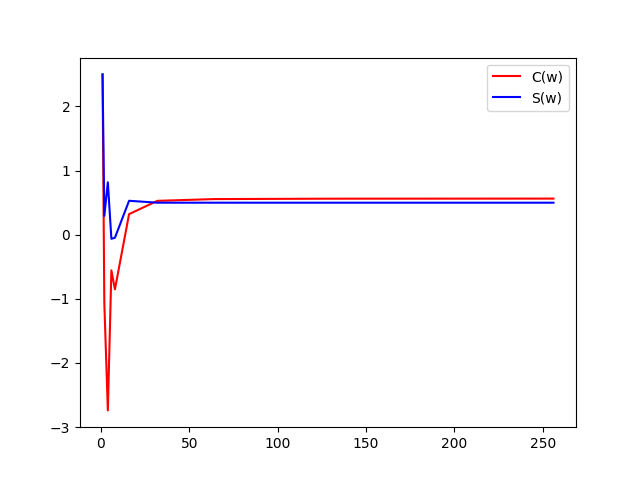
\includegraphics[width=\linewidth]{figures/ex1.png}
	\caption{Gráfica de C($\omega$) y S($\omega$) usando la regla del trapecio por cada $n$.}
	\label{fig:c_s_subdiv}
\end{figure}


\begin{table}[H]
	\centering
	\csvreader[
	tabular=|c|c|c|,
	table head=\hline \textbf{n} & \textbf{C($\omega$)} & \textbf{S($\omega$)} \\\hline,
	late after last line=\\\hline,
	]{data/c_s_subdivs.csv}{}{\csvlinetotablerow}
\end{table}

\paragraph{Discusión}

Vemos pues que los valores convergen, siendo bastante estables a partir $n = 32$.
